\documentclass[11pt]{article}

\usepackage[margin=1in]{geometry}
\usepackage{amsmath,amssymb}
\usepackage{xcolor}
\usepackage{tikz}
\usetikzlibrary{decorations.pathreplacing,arrows.meta,positioning}
\usepackage{booktabs}
\usepackage{tabularx}
\usepackage{enumitem}
\usepackage{graphicx}
\usepackage[colorlinks=true,allcolors=teal!55!black]{hyperref}

\definecolor{inkc}{HTML}{1B2433}
\definecolor{accentc}{HTML}{1F7A7C}
\definecolor{failc}{HTML}{C24A34}
\definecolor{successc}{HTML}{2F7D57}
\definecolor{mutedc}{HTML}{586274}

\newcommand{\cyes}{\textcolor{successc}{$\checkmark$}}
\newcommand{\cno}{\textcolor{failc}{$\times$}}
\newcommand{\rhat}{\hat r}
\newcommand{\arxiv}[1]{\href{https://arxiv.org/abs/#1}{arXiv:#1}}

\newcommand{\callout}[2]{%
  \par\smallskip\noindent
  \fcolorbox{accentc}{accentc!6}{%
    \begin{minipage}{\dimexpr\linewidth-2\fboxsep-2\fboxrule\relax}
      \textbf{\textcolor{accentc}{#1}}\;\; #2
    \end{minipage}}%
  \par\smallskip}

% skimmable one-look summary at the top of each idea
\newcommand{\glance}[4]{%
  \par\smallskip\noindent
  \fcolorbox{mutedc!45}{mutedc!8}{%
    \begin{minipage}{\dimexpr\linewidth-2\fboxsep-2\fboxrule\relax}
      \footnotesize
      \textbf{\textcolor{mutedc}{AT A GLANCE}}\\[3pt]
      \textbf{Q.}~#1\\[2pt]
      \textbf{How.}~#2\\[2pt]
      \textbf{Test.}~#3\\[2pt]
      \textbf{Why it matters.}~#4
    \end{minipage}}%
  \par\smallskip}

\setlength{\parskip}{0.5em}
\setlength{\parindent}{0pt}

\title{\textbf{Research Proposals}}
\author{Joseph M. Morante Jr.}
\date{September 5, 2026}

\begin{document}
\maketitle
\vspace{-1.5em}

% ==================================================================
\section{Reward-Model Uncertainty at the Top Tail}
% ==================================================================

\glance
  {Among a proxy reward model's top-rated answers, can the model's own \emph{uncertainty} flag the ones that are actually wrong?}
  {Score a fixed bank of answers, take the top tail (the answers a system would pick), and check whether uncertainty adds signal \emph{beyond} the score itself.}
  {$\Delta$AUROC $>0$ inside the selected tail, with score, length, and entropy already controlled --- and whether it depends on the judges being \emph{diverse}.}
  {Uncertainty-based safety filters act exactly on this selected set. If uncertainty fails here, they inherit the proxy's blind spots --- and that null is itself a safety-relevant result.}

\callout{Working claim.}{Optimization pressure against a proxy reward concentrates
selection on the proxy's own mistakes. This project tests whether reward-model
\emph{uncertainty} carries information about those mistakes---conditional on
selection, beyond the proxy score itself---and whether that information is a
property of ensemble \emph{diversity} rather than of ensembling per se.}

\callout{Research question.}{Among completions selected from the top tail of a
proxy reward model, do reward-model uncertainty estimates discriminate
gold-verified failures from successes \emph{beyond the proxy score itself}, and
how does this depend on \emph{ensemble diversity}?}

\textit{In plain terms.} The judge's favorite answers are a mix of real winners
and answers that fooled the judge. Among those favorites, does the judge's
confidence add anything the score didn't already say about which are fakes---and
does that depend on whether the panel of judges is near-clones or genuinely
different?

% ---------------- Figure 1 ----------------
\begin{figure}[t]\centering
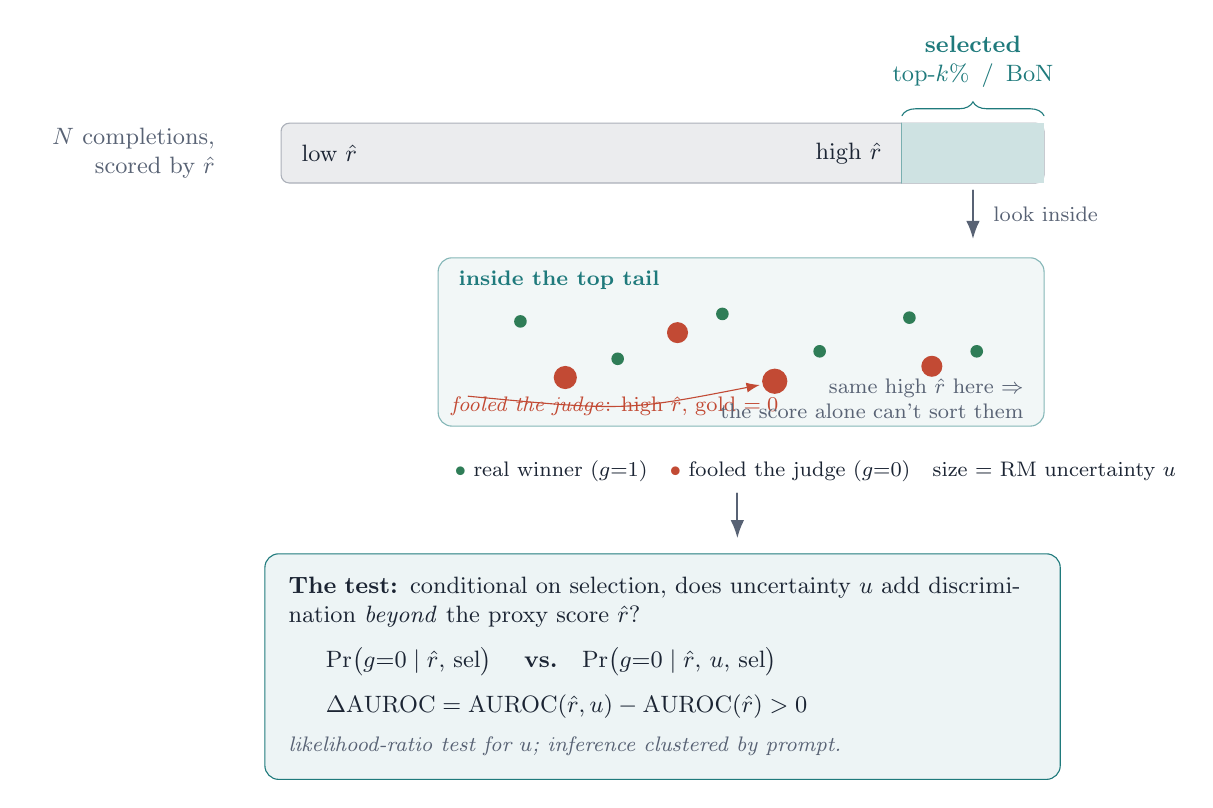
\begin{tikzpicture}[>=Latex, line cap=round, font=\small, inkc, scale=0.95, transform shape]
  \node[mutedc,anchor=east] at (-0.15,5.0) {\begin{tabular}{r}$N$ completions,\\ scored by $\rhat$\end{tabular}};
  \draw[rounded corners=3pt, fill=mutedc!12, draw=mutedc!50] (0.4,4.6) rectangle (10.6,5.4);
  \fill[accentc!22] (8.7,4.6) rectangle (10.6,5.4);
  \draw[accentc!60] (8.7,4.6) -- (8.7,5.4);
  \node[anchor=west] at (0.55,5.0) {low $\rhat$};
  \node[anchor=east] at (8.55,5.0) {high $\rhat$};
  \draw[decorate,decoration={brace,amplitude=5pt},accentc] (8.7,5.5) -- (10.6,5.5);
  \node[accentc,anchor=south,align=center] at (9.65,5.75){\textbf{selected}\\ top-$k\%$ \,/\, BoN};
  \draw[->,mutedc,thick] (9.65,4.5) -- (9.65,3.85);
  \node[mutedc,anchor=west,font=\footnotesize] at (9.8,4.18) {look inside};
  \draw[rounded corners=5pt, draw=accentc!55, fill=accentc!6] (2.5,1.35) rectangle (10.6,3.6);
  \node[accentc,anchor=north west,font=\footnotesize\bfseries] at (2.65,3.55) {inside the top tail};
  \foreach \p in {(3.6,2.75),(4.9,2.25),(6.3,2.85),(7.6,2.35),(8.8,2.8),(9.7,2.35)}
     \fill[successc] \p circle (2.4pt);
  \fill[failc] (4.2,2.0) circle (4.4pt);
  \fill[failc] (5.7,2.6) circle (4.0pt);
  \fill[failc] (7.0,1.95) circle (4.8pt);
  \fill[failc] (9.1,2.15) circle (4.0pt);
  \draw[failc,->] (2.9,1.75) .. controls (5.0,1.55) .. (6.8,1.9);
  \node[failc,anchor=west,font=\footnotesize,align=left] at (2.55,1.62){\emph{fooled the judge}: high $\rhat$, gold $=0$};
  \node[mutedc,anchor=east,font=\footnotesize,align=right] at (10.45,1.72){same high $\rhat$ here $\Rightarrow$\\ the score alone can't sort them};
  \node[anchor=west,font=\footnotesize] at (2.6,0.75)
    {\textcolor{successc}{$\bullet$} real winner ($g{=}1$)\quad
     \textcolor{failc}{$\bullet$} fooled the judge ($g{=}0$)\quad
     size $=$ RM uncertainty $u$};
  \draw[->,mutedc,thick] (6.5,0.45) -- (6.5,-0.15);
  \node[draw=accentc, rounded corners=5pt, fill=accentc!8, inner sep=9pt,
        align=left, text width=10.0cm, anchor=north] at (5.5,-0.35)
     {\textbf{The test:} conditional on selection, does uncertainty $u$ add
      discrimination \emph{beyond} the proxy score $\rhat$?\\[6pt]
      \hspace*{0.5cm}$\Pr\!\big(g{=}0 \mid \rhat,\,\mathrm{sel}\big)$
      \quad\textbf{vs.}\quad
      $\Pr\!\big(g{=}0 \mid \rhat,\, u,\,\mathrm{sel}\big)$\\[6pt]
      \hspace*{0.5cm}$\displaystyle \Delta\mathrm{AUROC}
        = \mathrm{AUROC}(\rhat, u) - \mathrm{AUROC}(\rhat) > 0$\\[4pt]
      {\footnotesize\color{mutedc}\itshape
      likelihood-ratio test for $u$; inference clustered by prompt.}};
\end{tikzpicture}
\caption{The top tail mixes true successes with completions that overrated the
proxy. The primary estimand asks whether reward-model uncertainty $u$
discriminates gold failures ($g{=}0$) from successes beyond the proxy score
$\rhat$, conditional on selection ($\Delta\mathrm{AUROC}>0$).}
\label{fig:toptail}
\end{figure}

\subsection{Background}
\begin{itemize}[leftmargin=1.2em,itemsep=3pt]
  \item \textbf{Optimizing against a proxy overfits its errors.} Best-of-$n$ and
    RLHF push a policy toward the \emph{maximum} of a learned reward, and the
    proxy--gold gap widens exactly where selection is strongest (Gao et al.,
    \arxiv{2210.10760}). Taking the argmax of an imperfect score is precisely the
    operation that surfaces its mistakes, so the winner set is enriched in them.
  \item \textbf{Reward-model uncertainty tracks reliability---but only
    unconditionally.} Ensemble and quantile-head uncertainty filters low-quality
    completions and improves BoN selection (URM/URME, \arxiv{2410.00847}), yet the
    result is reported \emph{marginally}---over the whole distribution, at seed-only
    diversity ($m{=}3$), and never conditioned on the proxy score inside the tail.
    That marginal effect is the published anchor this proposal extends.
  \item \textbf{Ensembles mitigate hacking, and diversity seems to matter.} RM
    ensembles reduce overoptimization (Coste et al., \arxiv{2310.02743}); ensemble
    \emph{diversity} (pretrain- vs finetune-seed) changes how much, though ensembles
    ``mitigate but do not eliminate'' hacking (Eisenstein et al., \arxiv{2312.09244}).
    Weight-averaging (WARM, \arxiv{2401.12187}) and uncertainty-aware training (UARM,
    \arxiv{2606.19818}; distributional / quantile RMs and their unifying lens,
    \arxiv{2606.09073}) all put uncertainty to work as \emph{mitigation during
    optimization}, not as a \emph{detector at the tail}.
  \item \textbf{Reward-model calibration is studied but coarse.} Uncertainty
    estimation for language reward models and its calibration were examined early
    (Gleave \& Irving, \arxiv{2203.07472}), without a selection-conditional,
    tail-local, beyond-score estimand.
  \item \textbf{Why the tail is the regime that matters.} Uncertainty-based
    safeguards (filtering, abstention, selective verification) operate on the
    \emph{selected} completions, where the proxy score is pinned near its ceiling
    (range restriction) and can no longer sort. Whether uncertainty helps
    \emph{there}, and \emph{beyond} the score, is the open and safety-relevant
    question.
\end{itemize}

\subsection{Gap / Novelty}
No published work evaluates \emph{selection-conditional, beyond-score} detection
\emph{at the tail}, gold-verified, with ensemble \emph{diversity manipulated and
mediated}. URM/URME is the closest result and sits at seed-only diversity with an
\emph{unconditional} estimand---this study either explains its headroom or bounds
its regime. The contribution is threefold and framed as tests: (i)~\emph{detection}
---does RM uncertainty carry failure information beyond the proxy score, conditional
on tail selection; (ii)~\emph{mechanism}---does ensemble diversity govern tail
detection via error decorrelation, separating ``more judges'' from ``different
judges''; (iii)~\emph{practice}---how much detection survives cheap estimators, and
what it buys in selective-verification budgets.

\subsection{Hypotheses}
\begin{description}[leftmargin=0em,itemsep=3pt]
  \item[H1 (incremental tail discrimination).] Conditional on tail selection,
    ensemble uncertainty adds discrimination beyond proxy score
    ($\Delta\text{AUROC}>0$, LR test)---and the increment shrinks as pressure grows
    (in $n$; as $k \to$ winner sets), because selection concentrates on shared
    blind spots.
  \item[H2 (diversity, mediated).] The increment rises along D1 $\to$ D2 $\to$ D3,
    mediated by error decorrelation (bank- and tail-measured): a diversity step that
    fails to decorrelate errors fails to raise $\Delta$AUROC.
  \item[H3 (pressure $\times$ diversity).] The decay of $\Delta$AUROC in $\log n$ is
    flatter for base-diverse ensembles: diversity buys robustness to optimization
    pressure, not just level.
  \item[H4 (cheap uncertainty).] Head/dropout/Laplace/quantile-width uncertainty is
    tested against true ensembles on the incremental estimand at the tail; parity and
    gap are both headlines.
  \item[H5 (failure taxonomy $+$ mechanism).] Discrimination is heterogeneous by
    failure class (extremal/format/length exploits vs shared-misconception reasoning
    errors), and per-class error correlation across ensemble members explains it:
    classes where diverse members fail independently are the classes uncertainty
    catches.
\end{description}
\textbf{Falsification remains informative.} H1 null even at D3/D4 $\to$
``beyond-score uncertainty carries no tail information---safeguards built on it
inherit the proxy's blind spots'' (the safety-relevant negative). H2 flat $\to$
diversity doesn't rescue detection. H1 holds, H3 fails $\to$ uncertainty helps only
under mild pressure; report the operating envelope.

\subsection{Formal Problem Definition and Mathematical Formulation}
\textbf{Setup.} For each prompt $x \in \mathcal{X}$, a fixed policy $\pi$ generates a
bank of $N$ completions, scored by proxy RM $\rhat$. Two tail constructions, both
reported: (a)~\emph{fixed-percent tails}---top $k\%$ of the bank ($k \in \{1,5,10\}$),
comparable across $n$; (b)~\emph{winner sets}---the actual BoN selections ($j{=}1$ per
draw) over draws of size $n \in \{16 \dots 4096\}$, the deployment-relevant set, with
optimization pressure
\[ \mathrm{KL} \;\approx\; \log n - \frac{n-1}{n}. \]
Gold $g(x,y) \in \{0,1\}$ labels tail members.

\textbf{Estimand (primary).} The incremental discrimination of uncertainty $u$ over
proxy score $\rhat$, \emph{conditional on selection}. Fit nested logistic models of
failure and compare them:
\[
\underbrace{\Pr\!\big(g{=}0 \mid \rhat,\ \mathrm{sel}\big)}_{\text{base}}
\qquad\text{vs.}\qquad
\underbrace{\Pr\!\big(g{=}0 \mid \rhat,\ u,\ \mathrm{sel}\big)}_{\text{full}},
\qquad
\Delta\mathrm{AUROC} = \mathrm{AUROC}(\rhat,u) - \mathrm{AUROC}(\rhat).
\]
Report $\Delta$AUROC, partial AUC, and the likelihood-ratio test for $u$, with
inference clustered by prompt. Unconditional tail AUROC is reported as a secondary,
comparable-to-prior-work number. The selection-induced correlation between $\rhat$
and $u$ inside the tail is itself reported (range-restriction diagnostic).

\textbf{Uncertainty estimators $u$.} \emph{Primary:} ensemble dispersion (std /
range / rank disagreement) over $\mathcal{E}=\{\rhat_1 \dots \rhat_m\}$. \emph{Cheap:}
multi-head, MC-dropout, last-layer/Laplace, quantile-head width. \emph{Trivial
covariates always in the model:} proxy score, length, policy token entropy.

\textbf{Diversity ladder $D$ (manipulated).} D1 seed / D2 data / D3 base /
D4 public-RM zoo, with diversity \emph{measured}: pairwise error correlation on gold
labels (full bank \emph{and} tail; tail-only is selection-biased), prediction
disagreement, and CKA. \textbf{Proxy quality} is a second manipulated covariate
(two training-data sizes, Stage 2), so discrimination is reported conditional on how
good the judge is.

\subsection{Design, Statistical Plan, and Experiment Matrix}
\textbf{Fractional design.} An anchor---D3, $m{=}4$, ensemble-std, $n{=}1024$,
$k{=}1\%$, verifiable gold, base proxy quality---plus one-factor-at-a-time sweeps;
the full factorial is not run. \textbf{Pre-registration:} primary endpoint is
$\Delta$AUROC at the anchor cell, D3 vs D1, clustered-bootstrap 95\% CI; all other
contrasts are secondary under Benjamini--Hochberg FDR. \textbf{Inference:} bootstrap
clustered by prompt and resampled over ensemble compositions; power target
$\ge\!\sim\!100$ failures and $100$ successes per primary cell for $\pm0.03$ AUROC CI.
\textbf{Confounds:} length and entropy always in the conditional model;
prompt-difficulty stratification; range-restriction diagnostic; gold-noise
sensitivity.

\renewcommand{\arraystretch}{1.2}
\begin{table}[h]\footnotesize\centering
\begin{tabularx}{\textwidth}{@{}l l X X l@{}}
\toprule
\textbf{ID} & \textbf{Question} & \textbf{Design} & \textbf{Metrics} & \textbf{Tier}\\
\midrule
E1 & Incremental tail discrimination (H1) & anchor $\pm$ pressure sweep ($n$, $k$, winner sets) & $\Delta$AUROC, partial AUC, LR test vs $n$, $k$ & Core\\
E2 & Diversity ladder $+$ mediation (H2) & $D$ sweep $\times\, m$ at anchor pressure & $\Delta$AUROC by $D$; error-correlation mediation & Core\\
E3 & Pressure $\times$ diversity (H3) & D1 vs D3 $\times$ full $n$ grid & slope of $\Delta$AUROC in $\log n$ by $D$ & Core\\
E4 & Cheap uncertainty (H4) & estimator sweep at anchor & incremental $\Delta$AUROC per estimator & Ablation\\
E5 & Taxonomy $+$ per-class mechanism (H5) & labeled tail failures at anchor \& deepest tail & per-class $\Delta$AUROC; per-class error corr. & Mechanism\\
E6 & Generality & anchor $+$ $D$ sweep under synthetic gold & cross-design agreement & Robustness\\
E7 & Selective verification (offline) & best cells; fixed-bank policy simulation & failures caught at $b\%$ budget; risk--coverage & Impact\\
E8 & Proxy quality & 2 quality levels $\times\ \{$D1, D3$\}$ & $\Delta$AUROC $\times$ proxy accuracy interaction & Stage-2\\
\bottomrule
\end{tabularx}
\end{table}

\subsection{Doubts / Risks}
\begin{itemize}[leftmargin=1.2em,itemsep=2pt]
  \item \textbf{The null is publishable and safety-relevant.} If $\Delta$AUROC
    $\approx 0$ even at D3/D4, that bounds uncertainty-based safeguards: they inherit
    the proxy's blind spots. Stage 0$+$1 already yield this paper if the effect is flat.
  \item \textbf{Range restriction is the core difficulty, not a nuisance.} Selection
    induces $\rhat$--$u$ dependence in the tail; the estimand is defined to absorb it
    (score always in both models) and the induced correlation is reported directly.
  \item \textbf{Mediation on the tail is selection-biased}---so error decorrelation is
    measured on the full bank as well, and both are reported.
  \item \textbf{E7 is offline only (scoped).} Adaptive verify-then-redraw loops create
    selection feedback a fixed bank cannot simulate; policy simulation is on the fixed
    bank in v1, with the representativeness caveat stated in limitations.
\end{itemize}

\subsection{Benchmarks}
\begin{itemize}[leftmargin=1.2em,itemsep=3pt]
  \item \textbf{MATH} (Hendrycks et al., \arxiv{2103.03874}) --- primary verifiable
    task: exact-match gold with the proxy trained \emph{without} gold access
    (weak-judge preference pairs). Stage 0 runs $\sim$200 prompts $\times\ N{=}4096$.
  \item \textbf{HumanEval} (\arxiv{2107.03374}) and \textbf{MBPP}
    (\arxiv{2108.07732}) --- code arm: unit-test pass/fail as gold, a second
    verifiable domain to check the estimand is not math-specific.
  \item \textbf{RewardBench} (\arxiv{2403.13787}) --- external reference for proxy-RM
    quality, anchoring the manipulated proxy-quality levels (E8) to a standard scale.
  \item \textbf{Synthetic-gold BoN protocol} (Gao-style, \arxiv{2210.10760}) ---
    open-ended generality (design~b): a large gold RM labels tail members, with a
    gold-noise sensitivity analysis.
\end{itemize}
Metrics reported throughout: $\Delta$AUROC and partial AUC (primary), LR test,
unconditional tail AUROC (secondary), per-class $\Delta$AUROC, error-correlation
mediation, and---for E7---failures caught at a $b\%$ verification budget with
risk--coverage curves.

\subsection{Positioning}
\begin{table}[h]\footnotesize\centering
\resizebox{\textwidth}{!}{%
\begin{tabular}{@{}l c c l c c c@{}}
\toprule
\textbf{Work} & \textbf{Tail} & \textbf{Gold} & \textbf{Uncertainty} &
\textbf{Beyond} & \textbf{Diversity} & \textbf{Taxonomy}\\
 & \textbf{focused} & \textbf{verified} & \textbf{as detector} &
\textbf{score} & \textbf{manipulated} & \\
\midrule
Gleave \& Irving '22 (\arxiv{2203.07472}) & \cno & \cno & calibration & \cno & observed & \cno\\
Gao et al. '22 (\arxiv{2210.10760}) & \cyes & \cyes\,synth & \cno & \cno & \cno & \cno\\
Coste et al. '23 (\arxiv{2310.02743}) & \cno & \cyes\,synth & mitigation & \cno & \cno & \cno\\
Eisenstein et al. '23 (\arxiv{2312.09244}) & partial & \cyes & mitigation & \cno & \cyes\,(2 lvl) & qual.\\
WARM (\arxiv{2401.12187}) & \cno & \cyes & merging & \cno & implicit & \cno\\
$\bullet$ URM/URME (\arxiv{2410.00847}) & \cno & \cno\,(BoN qual.) & \cyes\,uncond.\ filter & \cno & \cno\,(seed) & \cno\\
$\bullet$ UARM (\arxiv{2606.19818}) & \cno & \cno & mitigation (GRPO) & \cno & \cno & \cno\\
$\bullet$ Distributional RMs (\arxiv{2606.09073}) & \cno & \cno & theory/training & \cno & \cno & \cno\\
Lightweight-UQ / ADVPO (NeurIPS'24) & \cno & \cno & mitigation & \cno & \cno & \cno\\
\midrule
\textbf{This work} & \cyes & \cyes\,verif.$+$synth & \cyes & \cyes & \cyes\,4-lvl, mediated & \cyes\\
\bottomrule
\end{tabular}}
\end{table}
\textbf{Open cell:} selection-conditional, beyond-score detection at the tail,
gold-verified, with diversity manipulated and mediated.

\subsection{Value / Feasibility}
Runs entirely on frozen open models: one mid-size instruct policy; Bradley--Terry
proxy heads (gold withheld on verifiable tasks); the D4 zoo from public RMs; vLLM to
generate the bank once and reuse it; \emph{no RL anywhere}. The URM-style cheap
baseline adds only a quantile head (same data, different head). A single node
suffices. \textbf{Staged plan:} Stage 0 (vacuousness, power, confounds; gates on the
proxy--gold gap and covariate saturation) $\to$ Stage 1 (pre-registered anchor $+$
D-ladder; gate: any diversity signal promotes, flat yields a negative-result paper)
$\to$ Stage 2 (fractional matrix E1--E8, both gold designs, taxonomy labeling,
proxy-quality factor). Every branch produces a result.

% ==================================================================
\section{LOGIC Engine: Long-Output Generation Intelligent Caching Engine}
% ==================================================================

\glance
  {Can a reasoning model keep more of its useful ``thinking'' in memory by compressing \emph{smartly} instead of uniformly?}
  {Use attention entropy $H$ and compression distortion $D_{\mathrm{KL}}$ to spend full precision on \emph{logical anchors} and few bits on filler, all under a fixed \emph{average} bit budget.}
  {At matched budget \emph{and} GPU-hours, does adaptive precision beat static compression on final reasoning accuracy --- and is it \emph{where} the precision is spent that matters?}
  {More reasoning retained per GPU-hour means better --- and cheaper --- reasoning models, plus a mechanistic account of which tokens must stay pristine.}

\callout{Working claim.}{Reasoning models generate thousands of hidden ``thinking''
tokens, and uniform KV-cache compression destroys the few that carry the logic chain.
An entropy- and distortion-aware controller that spends full-precision cache on those
\emph{logical anchors} and compresses filler aggressively---under a \emph{matched}
average bit budget---should train a more accurate reasoner per GPU-hour than any
static rule.}

\textit{In plain terms.} Standard systems treat every part of an AI's short-term
memory the same. But some tokens hold a fragile chain of reasoning and some are
predictable filler. LOGIC Engine keeps a full-quality memory of the hard parts and
shrinks the easy parts, fitting more useful information on the same digital scratch
paper.

% ---------------- Figure 2 ----------------
\begin{figure}[t]\centering
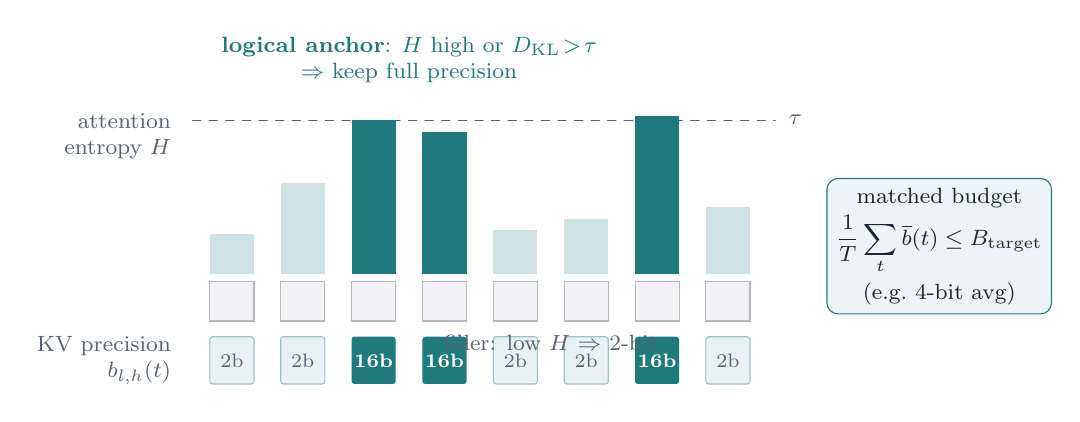
\begin{tikzpicture}[font=\small, inkc, >=Latex, line cap=round]
  % axis labels
  \node[mutedc,anchor=east,align=right,font=\footnotesize] at (-0.05,2.7) {attention\\ entropy $H$};
  % threshold
  \draw[dashed,mutedc] (0.1,2.9) -- (7.5,2.9);
  \node[mutedc,anchor=west,font=\footnotesize] at (7.55,2.9) {$\tau$};
  % entropy bars: (xcenter, height); base y=0.95 ; anchor if height>1.5
  \foreach \x/\hh/\isanchor in {0.6/0.5/0, 1.5/1.15/0, 2.4/1.95/1, 3.3/1.8/1, 4.2/0.55/0, 5.1/0.7/0, 6.0/2.0/1, 6.9/0.85/0}{
    \ifnum\isanchor=1
      \fill[accentc] (\x-0.28,0.95) rectangle (\x+0.28,{0.95+\hh});
    \else
      \fill[accentc!22] (\x-0.28,0.95) rectangle (\x+0.28,{0.95+\hh});
    \fi
    % token box
    \draw[mutedc!45,fill=mutedc!8] (\x-0.28,0.35) rectangle (\x+0.28,0.85);
    % KV precision block below
    \ifnum\isanchor=1
      \fill[accentc,rounded corners=1pt] (\x-0.28,-0.45) rectangle (\x+0.28,0.15);
      \node[white,font=\scriptsize\bfseries] at (\x,-0.15) {16b};
    \else
      \draw[accentc!45,fill=accentc!10,rounded corners=1pt] (\x-0.28,-0.45) rectangle (\x+0.28,0.15);
      \node[mutedc,font=\scriptsize] at (\x,-0.15) {2b};
    \fi
  }
  \node[mutedc,anchor=east,align=right,font=\footnotesize] at (-0.05,-0.15) {KV precision\\ $b_{l,h}(t)$};
  % callouts
  \node[accentc,anchor=south,align=center,font=\footnotesize] at (2.85,3.25)
      {\textbf{logical anchor}: $H$ high or $D_{\mathrm{KL}}\!>\!\tau$\\ $\Rightarrow$ keep full precision};
  \node[mutedc,anchor=north,align=center,font=\footnotesize] at (4.65,0.30)
      {filler: low $H$ $\Rightarrow$ 2-bit};
  % budget box
  \node[draw=accentc,rounded corners=4pt,fill=accentc!8,align=center,font=\footnotesize,
        anchor=west] at (8.15,1.3)
      {matched budget\\[2pt]
       $\dfrac{1}{T}\displaystyle\sum_t \overline{b}(t) \le B_{\mathrm{target}}$\\[2pt]
       (e.g.\ 4-bit avg)};
\end{tikzpicture}
\caption{LOGIC Engine allocates KV-cache precision per token, head, and layer from
attention entropy $H$ and the compression-induced distortion $D_{\mathrm{KL}}$: high-$H$
/ high-distortion \emph{logical anchors} keep full precision while predictable filler
is quantized hard, all under a fixed average bit budget $B_{\mathrm{target}}$.}
\label{fig:logic}
\end{figure}

\subsection{Background}
\begin{itemize}[leftmargin=1.2em,itemsep=3pt]
  \item \textbf{Attention is structurally heterogeneous, so uniform memory rules are
    wasteful.} Attention profiles differ sharply across heads and layers, and adaptive,
    structure-aware KV compression already beats uniform schemes (\textbf{FastGen},
    \arxiv{2310.01801}; \textbf{ARKV}, \arxiv{2603.08727}). A natural per-step measure of how ``focused''
    versus ``scattered'' a head is at generation step $t$ is the Shannon entropy of its
    attention distribution,
    \[ H\!\big(A^{(t)}_{l,h}\big) = -\sum_{i=1}^{t} P^{(t)}_{l,h}(i)\,\log_2 P^{(t)}_{l,h}(i), \tag{1}\]
    where $P^{(t)}_{l,h}(i)$ is the softmax attention on past token $i$. High entropy
    signals complex reasoning pathways whose compression risks breaking the logic chain;
    low entropy signals compressible, predictable text.
  \item \textbf{Reasoning models are different.} ``Thinking'' models emit thousands of
    hidden chain-of-thought tokens per problem, and uniform quantization silently erases
    vital intermediate clues (\textbf{R-KV}, \arxiv{2505.24133}; \textbf{LongFlow}, \arxiv{2603.11504}). Compression tuned for
    ordinary generation is not safe for a reasoning trace.
  \item \textbf{Logical anchors are measurable.} Recent frameworks quantify how much a
    head's attention \emph{distorts} when a memory block is compressed
    (\textbf{KVSculpt}, \arxiv{2603.27819}; \textbf{RLKV}, \arxiv{2510.08525}), via the KL divergence between the pristine
    and compressed attention maps,
    \[ D_{\mathrm{KL}}\!\big(P^{(t)}_{l,h}\,\|\,\tilde P^{(t)}_{l,h}\big)
       = \sum_{i=1}^{t} P^{(t)}_{l,h}(i)\,\log_2\!\frac{P^{(t)}_{l,h}(i)}{\tilde P^{(t)}_{l,h}(i)}. \tag{2}\]
    Tokens whose $D_{\mathrm{KL}}$ exceeds a safety threshold $\tau$ are flagged as
    \emph{logical anchors} and shielded from compression.
\end{itemize}

\subsection{Gap / Novelty}
Prior KV work is either \emph{static and uniform} (fixed-bit quantization, fixed-ratio
eviction) or \emph{structure-aware but not reasoning-budgeted} (FastGen/ARKV allocate by
attention pattern; R-KV/RLKV target reasoning redundancy). None combines
(i)~per-token/head/layer \emph{mixed-precision} allocation driven jointly by attention
\emph{entropy} and measured compression \emph{distortion}, (ii)~a hard \emph{matched
average-bit constraint} that makes an apples-to-apples comparison against static
compression possible, and (iii)~evaluation \emph{inside the RL training loop}, where
saved memory becomes more rollouts per GPU-hour and thus a better reasoner---not just a
smaller inference footprint.

\subsection{Hypothesis}
Managing memory dynamically---shrinking conversational filler to ultra-low bit widths
and reserving full precision for hard reasoning steps---lets the model retain more useful
information on the same scratch paper. Over a rollout of length $T$, the controller
enforces a strict matched average bit-rate across all layers $L$ and heads $H$:
\[
\frac{1}{T}\sum_{t=1}^{T}\Bigg[\frac{1}{|L|\,|H|}\sum_{l\in L}\sum_{h\in H} b_{l,h}(t)\Bigg]
\;\le\; B_{\mathrm{target}}, \tag{3}
\]
where $b_{l,h}(t)$ is the dynamic bit precision chosen at step $t$ and $B_{\mathrm{target}}$
is the controlled budget (e.g.\ exactly 4 bits). \textbf{H (main):} within a fixed
GPU-hour budget and at the same $B_{\mathrm{target}}$, entropy/KL-adaptive allocation
trains a more accurate reasoner than static compression. \textbf{H (mechanism):} the gain
comes from \emph{where and when} precision is spent---anchors identified by (1)--(2)---not
from a smaller footprint alone.

\subsection{Experiments}
\begin{enumerate}[leftmargin=1.4em,itemsep=2pt]
  \item \textbf{Adaptive vs.\ static at matched budget (headline).} Two identical
    reasoners, identical time/compute and identical \emph{average} bit budget
    $B_{\mathrm{target}}$: one under a rigid rule (uniform 4-bit quantization or
    fixed-ratio token eviction), one under LOGIC Engine. Compare final validation
    accuracy on hard reasoning suites, runtime, and training throughput.
  \item \textbf{Does the trigger actually add value? (mechanism / ablation).} Hold total
    memory matched, then flip the high-precision switch \emph{at random} for a control
    group; sweep the entropy and $D_{\mathrm{KL}}$ thresholds across layers. Test whether
    it is precisely \emph{where/when} LOGIC Engine allocates pristine memory that saves
    the reasoning trace---or whether gains are merely a reduced footprint. The honest
    null (entropy/KL do not localize what matters $\Rightarrow$ static is enough) is a
    publishable negative.
\end{enumerate}

\subsection{Doubts / Risks}
\begin{itemize}[leftmargin=1.2em,itemsep=2pt]
  \item \textbf{Measurement overhead is the central risk.} Computing per-head $H$, and
    especially $D_{\mathrm{KL}}$ (which needs a pristine-vs-compressed comparison), at
    every step can erase the savings. A cheap proxy or periodic re-estimation, charged
    honestly to the budget, is required.
  \item \textbf{Mixed-precision KV must be implementable in the serving stack.}
    Per-block variable bit-width on top of PagedAttention (``virtual precision paging'')
    needs kernel/paging support that does not negate throughput.
  \item \textbf{Matched-budget confound.} Average bits, GPU-hours, and wall-clock must all
    be held fixed, or apparent gains are footprint, not allocation---the ablation exists
    to detect exactly this.
  \item \textbf{Threshold transfer.} $\tau$ and entropy triggers may not transfer across
    layers or tasks; per-layer calibration and the threshold sweep address it.
\end{itemize}

\subsection{Benchmarks}
\begin{itemize}[leftmargin=1.2em,itemsep=3pt]
  \item \textbf{DeepSeek-R1 / OpenRLHF training benchmark} (\arxiv{2501.12948};
    OpenRLHF, \arxiv{2405.11143}) --- \emph{best fit}: a clean RL loop (GRPO/PPO, cf.\
    \arxiv{2402.03300}) under fixed time/space, to test whether smarter memory yields more
    thoughts per second and harder problems solved.
  \item \textbf{vLLM inference stack} (PagedAttention, \arxiv{2309.06180}) ---
    \emph{strongest real-world proof}: building dynamic virtual-precision paging on
    PagedAttention shows the engine works in production and cuts serving cost.
  \item \textbf{Open-R1 training stack} (Hugging Face open-source reproduction) ---
    \emph{scalability testbed}: verify that gains found on a small model hold when scaled
    to multi-billion-parameter reasoners.
\end{itemize}

\subsection{Value / Feasibility}
Runs on frozen open reasoning models with only a small allocation controller trained on
top; the heavy lifting is entropy/KL bookkeeping and quantized paging. A single node
suffices for the small-model study, with Open-R1 as the scale-up path. Deliverable: an
adaptive-precision KV cache that raises reasoning accuracy per GPU-hour at a fixed average
bit budget, with a mechanistic account (via entropy and $D_{\mathrm{KL}}$) of which tokens
must stay pristine.

% ==================================================================
\section*{References}
% ==================================================================
\small
\textit{Idea 1 --- reward-model uncertainty:}
\begin{itemize}[leftmargin=1.2em,itemsep=1pt]
  \item Gleave \& Irving. Uncertainty estimation for language reward models (2022). \arxiv{2203.07472}.
  \item Gao, Schulman \& Hilton. Scaling laws for reward model overoptimization (2022). \arxiv{2210.10760}.
  \item Coste et al. Reward model ensembles help mitigate overoptimization (2023). \arxiv{2310.02743}.
  \item Eisenstein et al. Helping or herding? Reward model ensembles mitigate but do not eliminate reward hacking (2023). \arxiv{2312.09244}.
  \item Ram\'e et al. WARM: On the benefits of weight averaged reward models (2024). \arxiv{2401.12187}.
  \item URM / URME: uncertainty-based reward modeling and filtering (ICLR 2025). \arxiv{2410.00847}.
  \item UARM: uncertainty-aware reward modeling (2026). \arxiv{2606.19818}.
  \item Distributional / quantile reward models; unifying lens (2026). \arxiv{2606.09073}.
  \item ADVPO / lightweight uncertainty quantification for RLHF (NeurIPS 2024).
  \item Hendrycks et al. MATH (2021). \arxiv{2103.03874}. \; Chen et al. HumanEval (2021). \arxiv{2107.03374}. \; Austin et al. MBPP (2021). \arxiv{2108.07732}. \; Lambert et al. RewardBench (2024). \arxiv{2403.13787}.
\end{itemize}
\textit{Idea 2 --- LOGIC Engine:}
\begin{itemize}[leftmargin=1.2em,itemsep=1pt]
  \item Ge et al. Model tells you what to discard: adaptive KV cache compression (FastGen) (2023). \arxiv{2310.01801}.
  \item ARKV: Adaptive and resource-efficient KV cache management under limited memory budget (2026). \arxiv{2603.08727}.
  \item R-KV: Redundancy-aware KV cache compression for reasoning models (2025). \arxiv{2505.24133}.
  \item LongFlow: Efficient KV cache compression for reasoning models (2026). \arxiv{2603.11504}.
  \item RLKV: Which heads matter for reasoning? RL-guided KV cache compression (2025). \arxiv{2510.08525}.
  \item KVSculpt: KV cache compression as distillation --- measures KL divergence between compressed-KV and full-cache outputs (2026). \arxiv{2603.27819}.
  \item DeepSeek-AI. DeepSeek-R1 (2025). \arxiv{2501.12948}. \; Hu et al. OpenRLHF (2024). \arxiv{2405.11143}. \; Shao et al. DeepSeekMath / GRPO (2024). \arxiv{2402.03300}.
  \item Kwon et al. Efficient memory management for LLM serving with PagedAttention (vLLM) (2023). \arxiv{2309.06180}. \; Hugging Face Open-R1 (open-source project).
\end{itemize}

\end{document}
